%%%%%%%%%%%%%%%%%%%%%%%%%%%%%%%%%%%%
% 配布用ハンドアウト（解答なし）
% コンパイルコマンド: lualatex chp7_handout.tex
%%%%%%%%%%%%%%%%%%%%%%%%%%%%%%%%%%%%

\documentclass[slidestop,compress,mathserif,handout]{beamer}

% 解答を非表示にする
\newcommand{\soln}[1]{ }
\newcommand{\solnGr}[1]{ }

% 4スライドを1ページに印刷する設定
\usepackage{pgfpages}
\pgfpagesuselayout{4 on 1}[a4paper,landscape,border shrink=5mm]

%%%%%%%%%%%%%%%%%%%%%%%%%%%%%%%%%%%%
% 日本語サポート（LuaLaTeX使用）
%%%%%%%%%%%%%%%%%%%%%%%%%%%%%%%%%%%%

\usepackage{luatexja}
\usepackage{luatexja-fontspec}

%%%%%%%%%%%%%%%%%%%%%%%%%%%%%%%%%%%%
% スタイル
%%%%%%%%%%%%%%%%%%%%%%%%%%%%%%%%%%%%

\input{../lec_style_JP}

% 配布用：練習問題の正解を通常アイテムとして表示（オーバーレイなし）
\renewcommand{\solnMult}[1]{\item #1}

\setbeamertemplate{footline}{%
  \insertframenumber\,/\,\inserttotalframenumber}

%%%%%%%%%%%%%%%%%%%%%%%%%%%%%%%%%%%%
% プリアンブル
%%%%%%%%%%%%%%%%%%%%%%%%%%%%%%%%%%%%

\title[第7章：数値データの推測]{第7章：数値データの推測}
\author{OpenIntro Statistics 第4版（日本語版）}
\institute{$\:$ \\ {\footnotesize 原著スライド：Mine \c{C}etinkaya-Rundel（OpenIntro）\\
\webLink{http://creativecommons.org/licenses/by-sa/3.0/us/}{CC BY-SA ライセンス}のもと使用・翻訳。\\
一部の画像はフェアユース（教育目的）に基づき使用。}}
\date{}

%%%%%%%%%%%%%%%%%%%%%%%%%%%%%%%%%%%%
% ドキュメント開始
%%%%%%%%%%%%%%%%%%%%%%%%%%%%%%%%%%%%

\begin{document}


%%%%%%%%%%%%%%%%%%%%%%%%%%%%%%%%%%%%
% タイトルページ
%%%%%%%%%%%%%%%%%%%%%%%%%%%%%%%%%%%%

{
\addtocounter{framenumber}{-1}
{\removepagenumbers
\usebackgroundtemplate{
\includegraphics[width=\paperwidth]{../OpenIntro_Grid_4_3-01.jpg}}
\begin{frame}

\hfill 
\includegraphics[width=20mm]{../oiLogo_highres}

\titlepage

\end{frame}
}
}


%%%%%%%%%%%%%%%%%%%%%%%%%%%%%%%%%%%%
% 各節
%%%%%%%%%%%%%%%%%%%%%%%%%%%%%%%%%%%%

%%%%%%%%%%%%%%%%%%%%%%%%%%%%%%%%%%%%

\section{$t$分布を用いた1標本平均の推測}

%%%%%%%%%%%%%%%%%%%%%%%%%%%%%%%%%%%%

\begin{frame}
\frametitle{13日の金曜日}

\dq{1990年から1992年にかけて、英国の研究者たちが13日の金曜日とその前週の金曜日（6日）の交通量、事故件数、入院件数に関するデータを収集した。以下は交通量に関するデータの抜粋である。場所1と場所2の交通量は独立であると仮定できる。}

{\scriptsize
\texttt{
\begin{center}
\begin{tabular}{rllrrrl}
  \hline
 & 種別 & 日付 & 6日 & 13日 & 差 & 場所  \\
  \hline
1 & 交通量 & 1990年7月 & 139246 & 138548 & 698 & 場所1 \\
  \rowcolor[gray]{.9}
  2 & 交通量 & 1990年7月 & 134012 & 132908 & 1104 & 場所2 \\
  3 & 交通量 & 1991年9月 & 137055 & 136018 & 1037 & 場所1 \\
  \rowcolor[gray]{.9}
  4 & 交通量 & 1991年9月 & 133732 & 131843 & 1889 & 場所2 \\
  5 & 交通量 & 1991年12月 & 123552 & 121641 & 1911 & 場所1 \\
  \rowcolor[gray]{.9}
  6 & 交通量 & 1991年12月 & 121139 & 118723 & 2416 & 場所2 \\
  7 & 交通量 & 1992年3月 & 128293 & 125532 & 2761 & 場所1 \\
  \rowcolor[gray]{.9}
  8 & 交通量 & 1992年3月 & 124631 & 120249 & 4382 & 場所2 \\
  9 & 交通量 & 1992年11月 & 124609 & 122770 & 1839 & 場所1 \\
  \rowcolor[gray]{.9}
  10 & 交通量 & 1992年11月 & 117584 & 117263 & 321 & 場所2 \\
   \hline
\end{tabular}
\end{center}
}}

\vfill

\rule{2.5cm}{0.25pt} \\
{\tiny Scanlon, T.J., Luben, R.N., Scanlon, F.L., Singleton, N. (1993), ``Is Friday the 13th Bad For Your Health?," BMJ, 307, 1584-1586.}

\end{frame}

%%%%%%%%%%%%%%%%%%%%%%%%%%%%%%%%%%%

\begin{frame}
\frametitle{13日の金曜日}

\begin{itemize}

\item 13日の金曜日と6日の金曜日で人々の行動が異なるかを調べたい。

\item 一つのアプローチは、この2つの日の交通量を比較することである。

\item $H_0:$ 6日と13日の金曜日の平均交通量は等しい。\\
$H_A:$ 6日と13日の金曜日の平均交通量は異なる。

\end{itemize}

$\:$ \\

\dq{データセットの各ケースは、同じ場所・同じ月・同じ年に記録された交通量を表している：6日の金曜日のカウントと13日の金曜日のカウントである。この2つのカウントは独立か？}

\soln{いいえ}

\end{frame}

%%%%%%%%%%%%%%%%%%%%%%%%%%%%%%%%%%%

\begin{frame}
\frametitle{仮説}

\pq{6日と13日の金曜日の平均交通量の差を検定するための仮説はどれか？}

\begin{enumerate}[(a)]
\item  \mathhl{H_0:} $\mu_{6th} = \mu_{13th}$ \\
\mathhl{H_A:} $\mu_{6th} \ne \mu_{13th}$
\item  \mathhl{H_0:} $p_{6th} = p_{13th}$ \\
\mathhl{H_A:} $p_{6th} \ne p_{13th}$
\solnMult{ \mathhl{H_0:} $\mu_{diff} = 0$ \\
\mathhl{H_A:} $\mu_{diff} \ne 0$ }
\item  \mathhl{H_0:} $\bar{x}_{diff} = 0$ \\
\mathhl{H_A:} $\bar{x}_{diff} = 0$
\end{enumerate}

\end{frame}

%%%%%%%%%%%%%%%%%%%%%%%%%%%%%%%%%%%

\begin{frame}
\frametitle{条件の確認}

\begin{itemize}

\item \hl{独立性：} ケース（行）は独立であると仮定する。

\item \hl{標本サイズ／歪み：} $\:$ \\

\twocol{0.75}{0.35}
{
{\tiny
\begin{itemize}

\item 標本分布は極端に歪んでいるようには見えないが、標本サイズが非常に小さいため判断が難しい。母集団分布が歪んでいるかどうかを考える必要がある――おそらく平均より交通量が少ない日と多い日は同程度に起こりうるため、歪んではいないだろう。

\item $\sigma$は未知であり、$n$が小さすぎるため$s$が$\sigma$の信頼できる推定値とは言えない。
\end{itemize}
}
}
{
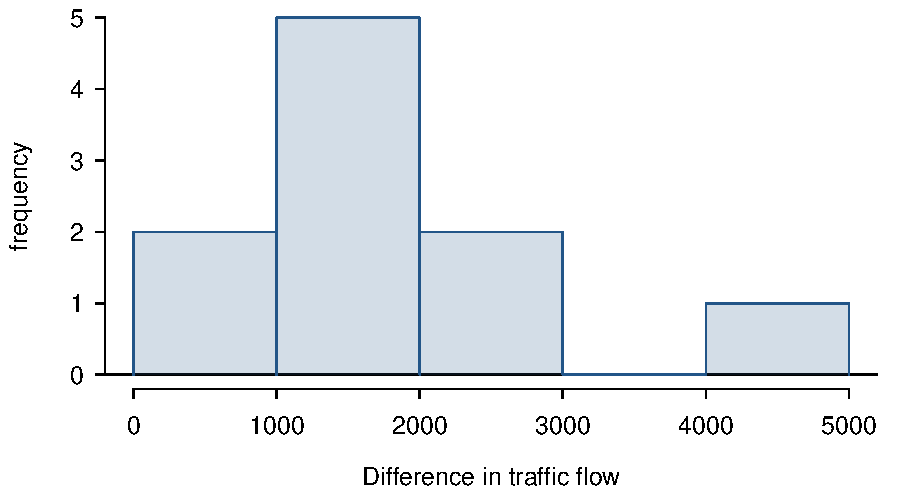
\includegraphics[width=\textwidth]{7-1_one_t/figures/friday/trafficHist}
}

\end{itemize}

$\:$ \\

\dq{では、標本サイズが小さい場合はどうすればよいか？}

\end{frame}

%%%%%%%%%%%%%%%%%%%%%%%%%%%%%%%%%%%

\begin{frame}
\frametitle{復習：大標本の役割}

観測値が独立であり、母集団分布が極端に歪んでいない限り、大標本によって次のことが保証される：

\begin{itemize}

\item 平均の標本分布がほぼ正規分布になる

\item 標準誤差の推定値$\frac{s}{\sqrt{n}}$が信頼できる

\end{itemize}

\end{frame}

%%%%%%%%%%%%%%%%%%%%%%%%%%%%%%%%%%%

\subsection{正規性の条件}

%%%%%%%%%%%%%%%%%%%%%%%%%%%%%%%%%%%

\begin{frame}
\frametitle{正規性の条件}

\begin{itemize}

\item 中心極限定理（CLT）によれば、母集団分布がほぼ正規であれば、\orange{いかなる}標本サイズでも標本分布はほぼ正規になる。

\item これは有用な特別なケースだが、小標本では正規性の確認が本質的に難しい。

\item 小標本における正規性の条件を確認する際は注意が必要である。データを調べるだけでなく、データの出所についても考えることが重要である。
\begin{itemize}
\item 例えば、この分布は対称であると期待できるか、また外れ値はまれであると確信できるか、という点を問うべきである。
\end{itemize}

\end{itemize}

\end{frame}

%%%%%%%%%%%%%%%%%%%%%%%%%%%%%%%%%%%

\subsection{$t$分布の紹介}

%%%%%%%%%%%%%%%%%%%%%%%%%%%%%%%%%%%

\begin{frame}
\frametitle{$t$分布}

\begin{itemize}

\item 母集団の標準偏差が未知の場合（ほぼ常にそうであるが）、標準誤差の推定の不確実性は\hl{$t$分布}という新しい分布を使用することで対処される。

\item この分布もベル形状をしているが、裾が正規分布より\hl{厚い}。

\item したがって、正規分布と比べて、平均から2SDを超える位置に観測値が落ちる可能性が高い。

\item 裾が厚いことは、標準誤差の推定が信頼性に欠ける場合（$n$が小さい場合）の問題を解決するのに役立つ。

\end{itemize}

\begin{center}
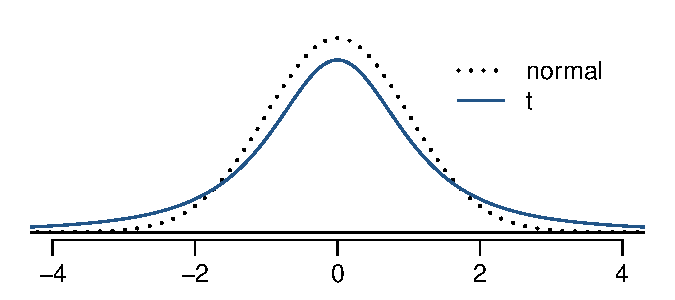
\includegraphics[width=0.5\textwidth]{7-1_one_t/figures/tDistCompareToNormalDist/tDistCompareToNormalDist}
\end{center}

\end{frame}

%%%%%%%%%%%%%%%%%%%%%%%%%%%%%%%%%%%

\begin{frame}
\frametitle{$t$分布（続き）}

\begin{itemize}

\item 標準正規（$z$）分布と同様に、常に0を中心とする。

\item パラメータは1つ：\hl{自由度}（\mathhl{df}）。

\end{itemize}

\begin{center}
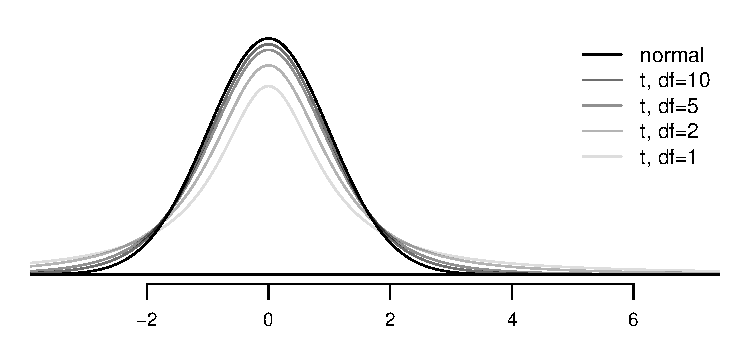
\includegraphics[width=0.8\textwidth]{7-1_one_t/figures/tDistConvergeToNormalDist/tDistConvergeToNormalDist}
\end{center}

\dq{$df$が増加すると$t$分布の形はどうなるか？}

\soln{正規分布に近づく。}

\end{frame}

%%%%%%%%%%%%%%%%%%%%%%%%%%%%%%%%%%%

\subsection{$t$分布を用いた仮説の検定}

%%%%%%%%%%%%%%%%%%%%%%%%%%%%%%%%%%%

\begin{frame}
\frametitle{13日の金曜日に戻ろう}

\vspace{-1cm}

{\footnotesize
\texttt{
\begin{center}
\begin{tabular}{rllrr || r || l}
  \hline
 & 種別 & 日付 & 6日 & 13日 & 差 & 場所  \\
  \hline
1 & 交通量 & 1990年7月 & 139246 & 138548 & 698 & 場所1 \\
  \rowcolor[gray]{.9}
  2 & 交通量 & 1990年7月 & 134012 & 132908 & 1104 & 場所2 \\
  3 & 交通量 & 1991年9月 & 137055 & 136018 & 1037 & 場所1 \\
  \rowcolor[gray]{.9}
  4 & 交通量 & 1991年9月 & 133732 & 131843 & 1889 & 場所2 \\
  5 & 交通量 & 1991年12月 & 123552 & 121641 & 1911 & 場所1 \\
  \rowcolor[gray]{.9}
  6 & 交通量 & 1991年12月 & 121139 & 118723 & 2416 & 場所2 \\
  7 & 交通量 & 1992年3月 & 128293 & 125532 & 2761 & 場所1 \\
  \rowcolor[gray]{.9}
  8 & 交通量 & 1992年3月 & 124631 & 120249 & 4382 & 場所2 \\
  9 & 交通量 & 1992年11月 & 124609 & 122770 & 1839 & 場所1 \\
  \rowcolor[gray]{.9}
  10 & 交通量 & 1992年11月 & 117584 & 117263 & 321 & 場所2 \\
   \hline
\end{tabular}
\end{center}
}}

\begin{align*}
\hspace{6cm} &\orange{$\bar{x}_{diff} = 1836$} \\
& \orange{$s_{diff} = 1176$} \\
& \orange{$n = 10$}
\end{align*}

\end{frame}

%%%%%%%%%%%%%%%%%%%%%%%%%%%%%%%%%%%

\begin{frame}
\frametitle{検定統計量の計算}

\formula{小標本平均の推測における検定統計量}
{小標本（$n < 30$）の平均に関する推測の検定統計量は、$df = n - 1$の$T$統計量である。
\[ T_{df} = \frac{\text{点推定量} - \text{帰無値}}{SE} \]}

\vspace{-0.5cm}

\hl{この文脈では…}
\begin{eqnarray*}
\text{点推定量} &=& \bar{x}_{diff} = 1836 \\
SE &=& \frac{s_{diff}}{\sqrt{n}} = \frac{1176}{\sqrt{10}} = 372 \\
T &=& \frac{1836 - 0}{372} = 4.94 \\
df &=& 10 - 1 = 9
\end{eqnarray*}

\vspace{-0.25cm}

\Note{帰無仮説で$\mu_{diff} = 0$と設定したため、帰無値は0である。}

\end{frame}

%%%%%%%%%%%%%%%%%%%%%%%%%%%%%%%%%%%

\begin{frame}[fragile]
\frametitle{p値の計算}

\begin{itemize}

\item p値は、再び$t$分布の裾の面積として計算される。

\item Rを使う場合：
\begin{verbatim}
> 2 * pt(4.94, df = 9, lower.tail = FALSE)

[1] 0.0008022394
\end{verbatim}

\item ウェブアプリを使う場合：

\href{https://gallery.shinyapps.io/dist_calc/}{\textcolor{oiB}{https://gallery.shinyapps.io/dist\_calc/}}

\item これらが利用できない場合は、$t$表を使うことができる。

\end{itemize}

\end{frame}

%%%%%%%%%%%%%%%%%%%%%%%%%%%%%%%%%%%


\begin{frame}
\frametitle{検定の結論}

\dq{この仮説検定の結論は何か？}

p値が非常に小さいため、データは6日と13日の金曜日の交通量に差があることを示す強い証拠を提供していると結論付ける。

\end{frame}

%%%%%%%%%%%%%%%%%%%%%%%%%%%%%%%%%%%%

\subsection{$t$分布を用いた信頼区間の構築}

%%%%%%%%%%%%%%%%%%%%%%%%%%%%%%%%%%%

\begin{frame}
\frametitle{差はどれくらいか？}

\begin{itemize}

\item 6日と13日の金曜日の交通量に差があると結論付けた。

\item しかし、その差が具体的にどれくらいかを知ることがより興味深い。

\item 信頼区間を使ってこの差を推定することができる。

\end{itemize}

\end{frame}

%%%%%%%%%%%%%%%%%%%%%%%%%%%%%%%%%%%

\begin{frame}
\frametitle{小標本平均の信頼区間}

\begin{itemize}

\item 信頼区間は常に次の形をとる：
\[ \text{点推定量} \pm {ME} \]

\item MEは常に、臨界値と標準誤差の積として計算される。

\item 小標本平均は$z$分布ではなく$t$分布に従うため、臨界値は$t^\star$（$z^\star$ではなく）となる：
\[ \text{点推定量} \pm t^{\star} \times SE \]

\end{itemize}

\end{frame}

%%%%%%%%%%%%%%%%%%%%%%%%%%%%%%%%%%%

\begin{frame}[fragile]
\frametitle{臨界値$t^\star$の計算}


Rを使う場合：
\begin{verbatim}

> qt(p = 0.975, df = 9)

[1] 2.262157

\end{verbatim}

\end{frame}

%%%%%%%%%%%%%%%%%%%%%%%%%%%%%%%%%%%

\begin{frame}
\frametitle{小標本平均の信頼区間の構築}

\pq{6日と13日の金曜日の交通量の差に対する95\%信頼区間の正しい計算はどれか？}
\[ \bar{x}_{diff} = 1836 \qquad s_{diff} = 1176 \qquad n = 10 \qquad SE = 372 \]

\twocol{0.35}{0.65}
{
\begin{enumerate}[(a)]

\item $1836 \pm 1.96 \times 372$

\solnMult{ $1836 \pm 2.26 \times 372$}

\item $1836 \pm -2.26 \times 372$

\item $1836 \pm 2.26 \times 1176$

\end{enumerate}
}
{
\only<2->{\orange{$\rightarrow$ (995, 2677)}}
\vspace{0.25cm}
}

\end{frame}

%%%%%%%%%%%%%%%%%%%%%%%%%%%%%%%%%%%

\begin{frame}
\frametitle{信頼区間の解釈}

\pq{先ほど計算した信頼区間の\orange{最も適切な}解釈はどれか？
\[ \mu_{diff: 6th - 13th} = (995, 2677) \]
}

95\%の確率で…

\begin{enumerate}[(a)]

\item 6日と13日の金曜日の平均交通量の差は995台から2,677台の間にある。

\item 6日の金曜日の方が13日の金曜日より平均して995台から2,677台少ない車が走っている。

\item 6日の金曜日の方が13日の金曜日より平均して995台少ないから2,677台多い車が走っている。

\solnMult{ 13日の金曜日の方が6日の金曜日より平均して995台から2,677台少ない車が走っている。}

\end{enumerate}

\end{frame}

%%%%%%%%%%%%%%%%%%%%%%%%%%%%%%%%%%%

\subsection{まとめ}

%%%%%%%%%%%%%%%%%%%%%%%%%%%%%%%%%%%

\begin{frame}
\frametitle{まとめ}

\dq{仮説検定の結論は信頼区間の結果と一致しているか？}

$\:$ \\

\soln{はい、仮説検定で有意な差が見られ、信頼区間は帰無値0を含んでいない。}

$\:$ \\

\dq{この研究の結果は、人々が13日の金曜日を不吉な日だと信じていることを示唆しているか？}

$\:$ \\

\soln{いいえ、これは観察研究である。この2日間の道路上の車の台数に有意な差があることを観察したに過ぎない。人々の信念を検定したわけではない。}

\end{frame}

%%%%%%%%%%%%%%%%%%%%%%%%%%%%%%%%%%%

\begin{frame}
\frametitle{まとめ：$t$分布を用いた推測}

\begin{itemize}

\item $\sigma$が未知の場合は、$SE = \frac{s}{\sqrt{n}}$として$t$分布を使用する。

\item 条件：
\begin{itemize}
\item 観測値の独立性（ランダム標本により確認、非復元抽出の場合は$n < $母集団の10\%）
\item 極端な歪みがない
\end{itemize}

\item 仮説検定：
\[ T_{df} = \frac{\text{点推定量} - \text{帰無値}}{SE}\text{，ただし }df = n - 1 \]

\item 信頼区間：$\text{点推定量} \pm t_{df}^\star \times SE$

\end{itemize}

\vspace{-0.25cm}

\Note{ここで使った例は対データの平均（従属グループ間の差）に関するものであった。観測値の差を取り、その差だけ（1標本）を分析に使用したため、1標本の場合と同じ手順となる。}

\end{frame}

%%%%%%%%%%%%%%%%%%%%%%%%%%%%%%%%%%%

%%%%%%%%%%%%%%%%%%%%%%%%%%%%%%%%%%%%

\section{対データ}

%%%%%%%%%%%%%%%%%%%%%%%%%%%%%%%%%%%

\subsection{対になった観測値}

\begin{frame}

\dq{「高校とその先」調査から200人の観測値が無作為に抽出された。同じ生徒が読解テストと作文テストを受け、そのスコアを以下に示す。一見して、読解と作文のテストスコアの平均に差があるように見えるか？}

\begin{center}
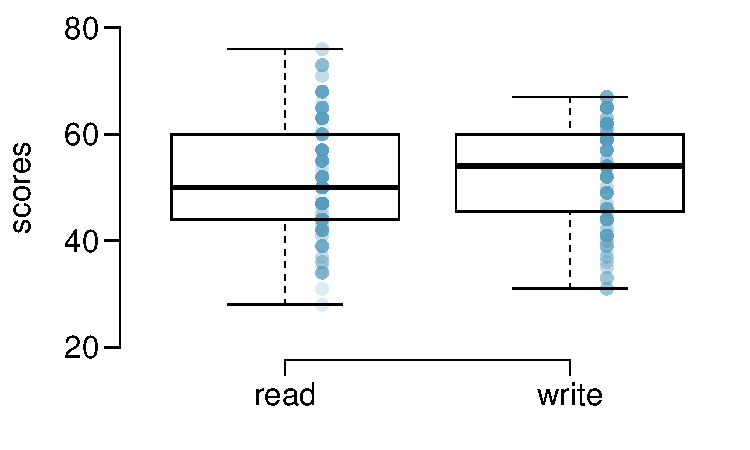
\includegraphics[width=0.5\textwidth]{7-2_paired/figures/hsb2/hsb2_read_write_box}
\end{center}

\end{frame}

%%%%%%%%%%%%%%%%%%%%%%%%%%%%%%%%%%%%

\begin{frame}

\pq{同じ生徒が読解テストと作文テストを受け、そのスコアを以下に示す。各生徒の読解スコアと作文スコアは互いに独立か？}

{\small
\begin{center}
\begin{tabular}{rrrr}
  \hline
 & id & 読解 & 作文 \\
  \hline
1 & 70 & 57 & 52 \\
  2 & 86 & 44 & 33 \\
  3 & 141 & 63 & 44 \\
  4 & 172 & 47 & 52 \\
  $\vdots$ &   $\vdots$  &   $\vdots$ &   $\vdots$  \\
  200 & 137 & 63 & 65 \\
   \hline
\end{tabular}
\end{center}
}

\begin{multicols}{2}
\begin{enumerate}[(a)]
\item はい
\solnMult{いいえ}
\end{enumerate}
\end{multicols}

\end{frame}

%%%%%%%%%%%%%%%%%%%%%%%%%%%%%%%%%%%%

\begin{frame}
\frametitle{対データの分析}

\begin{itemize}

\item 2組の観測値がこのような特別な対応関係（独立でない）を持つとき、それらは\hl{対データ}と呼ばれる。

\item 対データを分析するには、各ペアの観測値の結果の差を見ることが有用である。
\[ \text{差} = \text{読解} - \text{作文} \]

\item 常に一貫した順序で引き算することが重要である。

\end{itemize}

\twocol{0.5}{0.5}{
{\small
\begin{center}
\begin{tabular}{rrrr >{\columncolor[gray]{.9}}r}
  \hline
 & id & 読解 & 作文 & 差 \\
  \hline
1 & 70 & 57 & 52 & 5 \\
  2 & 86 & 44 & 33 & 11 \\
  3 & 141 & 63 & 44 & 19 \\
  4 & 172 & 47 & 52 & -5 \\
  $\vdots$ &   $\vdots$  &   $\vdots$ &   $\vdots$ &   $\vdots$ \\
  200 & 137 & 63 & 65 & -2 \\
   \hline
\end{tabular}
\end{center}
}
}
{
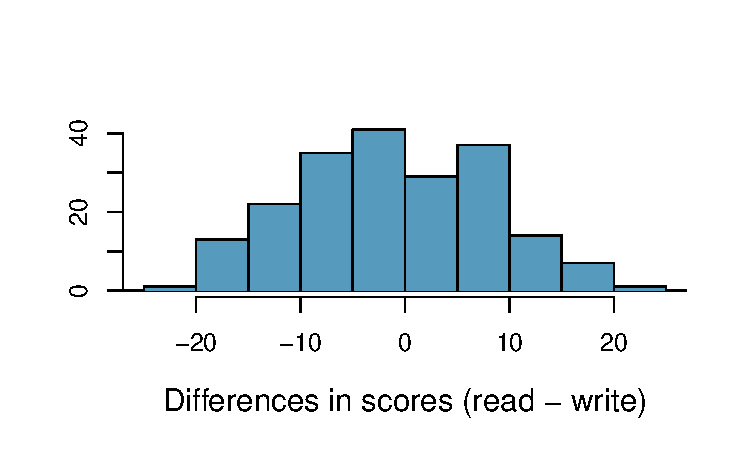
\includegraphics[width=\textwidth]{7-2_paired/figures/hsb2/hsb2_diff_hist}
}

\end{frame}

%%%%%%%%%%%%%%%%%%%%%%%%%%%%%%%%%%%%

\begin{frame}
\frametitle{母数と点推定量}

\begin{itemize}

\item \hl{関心のある母数：}\orange{すべての}高校生の読解スコアと作文スコアの平均差。
\[ \mu_{diff} \]

$\:$ \\

\item \hl{点推定量：}\orange{標本として抽出された}高校生の読解スコアと作文スコアの平均差。
\[ \bar{x}_{diff} \]

\end{itemize}

\end{frame}

%%%%%%%%%%%%%%%%%%%%%%%%%%%%%%%%%%%%

\subsection{対データの推測}

\begin{frame}
\frametitle{仮説の設定}

\dq{読解と作文の試験のスコアに実際に差がないとすれば、平均差はどれくらいと期待されるか？}

\soln{0}

$\:$ \\

\dq{読解と作文の平均スコアに差があるかどうかを検定するための仮説は何か？}

\begin{itemize}
\item[$H_0$:] 読解と作文の平均スコアに差はない。
\[ \mu_{diff} = 0 \]
\item[$H_A$:] 読解と作文の平均スコアに差がある。
\[ \mu_{diff} \ne 0 \]
\end{itemize}

\end{frame}

%%%%%%%%%%%%%%%%%%%%%%%%%%%%%%%%%%%%

\begin{frame}
\frametitle{新しいことは何もない}

\begin{itemize}

\item 分析はこれまでと何ら変わりない。

\item \orange{1つの}標本のデータ（差）を持っている。

\item 平均差が0と異なるかどうかを検定する。

\end{itemize}

\end{frame}

%%%%%%%%%%%%%%%%%%%%%%%%%%%%%%%%%%%%

\begin{frame}
\frametitle{仮定と条件の確認}

\pq{正しいのはどれか？}

\begin{enumerate}[(a)]
\solnMult{生徒は無作為に抽出され、全高校生の10\%未満であるため、標本中のある生徒の読解スコアと作文スコアの差は別の生徒の差と独立であると仮定できる。}
\item 差の分布が二峰性であるため、仮説検定を続けることができない。
\item 差をランダムにするには復元抽出で標本を取るべきであった。
\item 生徒は無作為に抽出され、全生徒の10\%未満であるため、平均差の標本分布はほぼ正規分布になると仮定できる。
\end{enumerate}

\end{frame}

%%%%%%%%%%%%%%%%%%%%%%%%%%%%%%%%%%%

\begin{frame}[shrink]
\frametitle{検定統計量とp値の計算}

\dq{2つのテストの観測された平均スコア差は$-0.545$点、差の標準偏差は$8.887$点であった。$\alpha = 0.05$として、このデータは2つの試験の平均スコアに差があることの説得力ある証拠を提供しているか？}

\twocol{0.5}{0.5}
{
\begin{center}
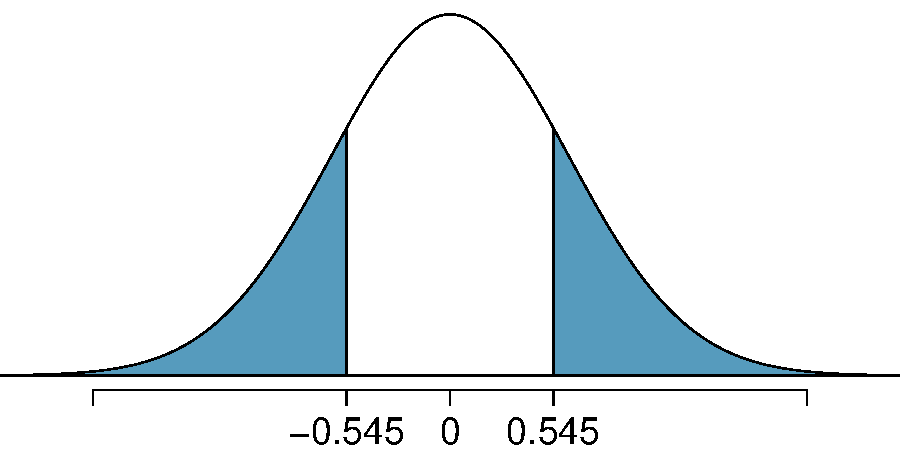
\includegraphics[width=\textwidth]{7-2_paired/figures/hsb2/hsb2_read_write_pval}
\end{center}
}
{
\begin{eqnarray*}
T &=& \frac{-0.545 - 0}{\frac{8.887}{\sqrt{200}}} \\
&=& \frac{-0.545}{0.628} = -0.87 \\
df &=& 200 - 1 = 199 \\
p\text{値} &=& 0.1927 \times 2 = 0.3854
\end{eqnarray*}
}

$\:$ \\
p値$>$0.05であるため、帰無仮説を棄却できない。データは読解と作文の平均スコアに差があることの説得力ある証拠を\underline{提供していない}。

\end{frame}

%%%%%%%%%%%%%%%%%%%%%%%%%%%%%%%%%%%

\begin{frame}
\frametitle{p値の解釈}

\pq{p値の正しい解釈はどれか？}

\begin{enumerate}[(a)]
\item 読解と作文の平均スコアが等しい確率。
\item 読解と作文の平均スコアが異なる確率。
\solnMult{真の平均差が0であると仮定したとき、200人の学生の無作為標本において読解と作文スコアの平均差が（いずれかの方向に）少なくとも0.545となる確率。}
\item 帰無仮説が真であるときに誤って帰無仮説を棄却する確率。
\end{enumerate}

\end{frame}

%%%%%%%%%%%%%%%%%%%%%%%%%%%%%%%%%%%%

\begin{frame}
\frametitle{仮説検定 $\leftrightarrow$ 信頼区間}

\pq{読解と作文スコアの平均差に対する95\%信頼区間を構築するとした場合、この区間は0を含むと期待されるか？}

\begin{enumerate}[(a)]
\solnMult{はい}
\item いいえ
\item 与えられた情報からは判断できない
\end{enumerate}

\soln{
\begin{eqnarray*}
-0.545 \pm 1.97 \frac{8.887}{\sqrt{200}} &=& -0.545 \pm 1.97 \times 0.628 \\
&=& -0.545 \pm 1.24 \\
&=& (-1.785, 0.695)
\end{eqnarray*}
}

\end{frame}

%%%%%%%%%%%%%%%%%%%%%%%%%%%%%%%%%%%%

%%%%%%%%%%%%%%%%%%%%%%%%%%%%%%%%%%%%

\section{2つの平均の差}

%%%%%%%%%%%%%%%%%%%%%%%%%%%%%%%%%%%%

\begin{frame}
\frametitle{ダイヤモンド}

\begin{itemize}

\item ダイヤモンドの重さはカラット（carat）で測る。

\item 1カラット＝100ポイント、0.99カラット＝99ポイント、など。

\item 0.99カラットのダイヤモンドと1カラットのダイヤモンドのサイズの違いは肉眼では識別できないが、1カラットのダイヤモンドの価格は0.99カラットのダイヤモンドより高い傾向があるだろうか？

\item 0.99カラットと1カラットのダイヤモンドの平均価格に差があるかどうかを検定する。

\item 同等の単位で比較できるよう、0.99カラットのダイヤモンドの価格を99で、1カラットのダイヤモンドの価格を100で割り、平均ポイント価格を比較する。

\end{itemize}

\hfill 
\includegraphics[width=0.2\textwidth]{7-3_diff_two_mean/figures/diamonds/diamond}

\end{frame}

%%%%%%%%%%%%%%%%%%%%%%%%%%%%%%%%%%%

\begin{frame}[fragile]
\frametitle{データ}

\begin{center}
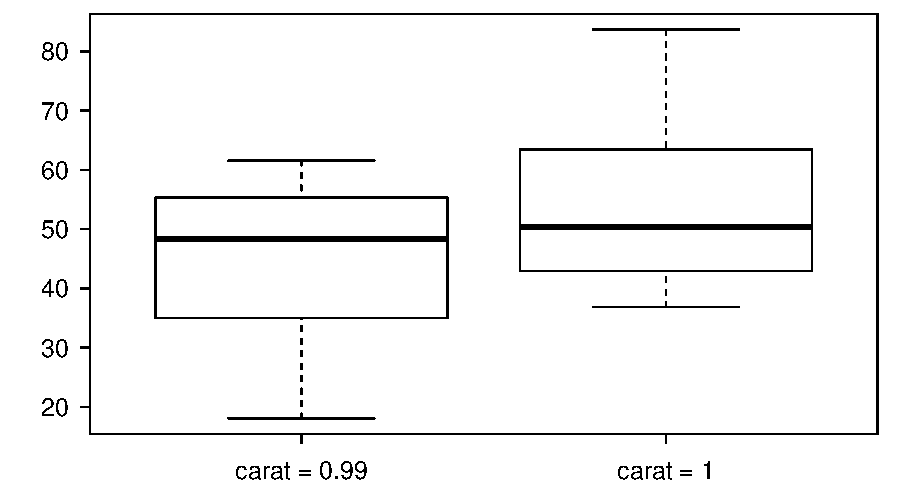
\includegraphics[width=0.55\textwidth]{7-3_diff_two_mean/figures/diamonds/diamondBox.pdf}
\end{center}

{\small
\begin{center}
\begin{tabular}{l | c | c}
		& {\footnotesize \hl{0.99カラット}} &  {\footnotesize \hl{1カラット}}  \\
		& pt99	& pt100 \\
\hline
$\bar{x}$	& 44.50		& 53.43 \\
$s$		& 13.32		& 12.22 \\
$n$		& 23			& 30
\end{tabular}
\end{center}
}

\Note{このデータは\texttt{ggplot2} Rパッケージのダイヤモンドデータセットからのランダムサンプルである。}

\end{frame}

%%%%%%%%%%%%%%%%%%%%%%%%%%%%%%%%%%%

\begin{frame}
\frametitle{母数と点推定量}

\begin{itemize}

\item \hl{関心のある母数：}\orange{すべての}0.99カラットと1カラットのダイヤモンドのポイント価格の平均差。
\[ \mu_{pt99} - \mu_{pt100} \]

$\:$ \\

\item \hl{点推定量：}\orange{標本として抽出された}0.99カラットと1カラットのダイヤモンドのポイント価格の平均差。
\[ \bar{x}_{pt99} - \bar{x}_{pt100} \]

\end{itemize}

\end{frame}

%%%%%%%%%%%%%%%%%%%%%%%%%%%%%%%%%%%

\begin{frame}
\frametitle{仮説}

\pq{1カラットのダイヤモンドの平均ポイント価格（$_{pt100}$）が0.99カラットの平均ポイント価格（$_{pt99}$）より高いかどうかを検定するための正しい仮説の組合せはどれか？}

\begin{enumerate}[(a)]

\item  \mathhl{H_0:} $\mu_{pt99} = \mu_{pt100}$ \\
\mathhl{H_A:} $\mu_{pt99} \ne \mu_{pt100}$

\item  \mathhl{H_0:} $\mu_{pt99} = \mu_{pt100}$ \\
\mathhl{H_A:} $\mu_{pt99} > \mu_{pt100}$

\solnMult{  \mathhl{H_0:} $\mu_{pt99} = \mu_{pt100}$ \\
\mathhl{H_A:} $\mu_{pt99} < \mu_{pt100}$ }

\item  \mathhl{H_0:} $\bar{x}_{pt99} = \bar{x}_{pt100}$ \\
\mathhl{H_A:} $\bar{x}_{pt99} < \bar{x}_{pt100}$

\end{enumerate}

\end{frame}

%%%%%%%%%%%%%%%%%%%%%%%%%%%%%%%%%%%

\begin{frame}
\frametitle{条件の確認}

\pq{理論的手法でこの仮説検定を行うために満たす必要が\underline{ない}条件はどれか？}

\begin{enumerate}[(a)]

\item 標本中の0.99カラットのダイヤモンド同士は独立、1カラットのダイヤモンド同士も独立でなければならない。

\item 標本中の0.99カラットと1カラットのダイヤモンドのポイント価格は独立でなければならない。

\item 0.99カラットと1カラットのダイヤモンドのポイント価格の分布は極端に歪んでいてはならない。

\solnMult{両グループの標本サイズはそれぞれ少なくとも30でなければならない。}

\end{enumerate}

\end{frame}

%%%%%%%%%%%%%%%%%%%%%%%%%%%%%%%%%%%%

\subsection{2つの平均の差の標本分布}

%%%%%%%%%%%%%%%%%%%%%%%%%%%%%%%%%%%%

\begin{frame}
\frametitle{検定統計量}

\formula{2つの小標本平均の差に関する推測の検定統計量}
{$\sigma_1$と$\sigma_2$が未知の場合、2つの平均の差に関する推測の検定統計量は$T$統計量である。
\[ T_{df} = \frac{\text{点推定量} - \text{帰無値}}{SE} \]
ただし
\[ SE = \sqrt{ \frac{s_1^2}{n_1} + \frac{s_2^2}{n_2} } \qquad \text{ および } \qquad df = \min(n_1 - 1, n_2 - 1) \]
}

\Note{$df$の計算は実際にははるかに複雑である。手計算の場合は上の式を使って真の$df$を\underline{推定}する。}

\end{frame}

%%%%%%%%%%%%%%%%%%%%%%%%%%%%%%%%%%%%

\subsection{2つの平均の差の仮説検定}

%%%%%%%%%%%%%%%%%%%%%%%%%%%%%%%%%%%%

\begin{frame}
\frametitle{検定統計量（続き）}

{\small
\begin{center}
\begin{tabular}{l | c | c}
		& {\footnotesize \hl{0.99カラット}} &  {\footnotesize \hl{1カラット}}  \\
		& pt99	& pt100 \\
\hline
$\bar{x}$	& 44.50		& 53.43 \\
$s$		& 13.32		& 12.22 \\
$n$		& 23			& 30
\end{tabular}
\end{center}
}

\hl{この文脈では…}

{\small
\begin{eqnarray*}
T &=& \frac{\text{点推定量} - \text{帰無値} }{SE} \\
&=& \frac{(44.50 - 53.43) - 0}{ \sqrt{\frac{13.32^2}{23} + \frac{12.22^2}{30} }} \\
&=& \frac{-8.93}{3.56} \\
&=& -2.508
\end{eqnarray*}
}

\end{frame}

%%%%%%%%%%%%%%%%%%%%%%%%%%%%%%%%%%%%

\begin{frame}
\frametitle{検定統計量（続き）}

\pq{この仮説検定の正しい$df$はどれか？}

\twocol{0.3}{0.7}
{
\begin{enumerate}[(a)]
\solnMult{ 22 }
\item 23
\item 30
\item 29
\item 52
\end{enumerate}
}
{
\soln{
\orange{$\rightarrow df = \min(n_{pt99} - 1, n_{pt100} - 1)$ \\
$= \min(23 - 1, 30 - 1)$ \\
$= \min(22,29) = 22$} \\
\vspace{1cm}
}}

\end{frame}

%%%%%%%%%%%%%%%%%%%%%%%%%%%%%%%%%%%%

\begin{frame}[fragile]
\frametitle{p値}

\pq{この仮説検定の正しいp値はどれか？}

\[ T = -2.508 \qquad df = 22 \]

\begin{enumerate}[(a)]
\item 0.005から0.01の間
\solnMult{0.01から0.025の間}
\item 0.02から0.05の間
\item 0.01から0.02の間
\end{enumerate}

\begin{verbatim}
> pt(q = -2.508, df = 22)
[1] 0.0100071
\end{verbatim}

\end{frame}

%%%%%%%%%%%%%%%%%%%%%%%%%%%%%%%%%%%%

\begin{frame}
\frametitle{まとめ}

\dq{仮説検定の結論は何か？ダイヤモンドを購入する際に、この結論はあなたの行動をどのように変えるか？}


\soln{
\begin{itemize}
\item p値が小さいため$H_0$を棄却する。データは0.99カラットのダイヤモンドのポイント価格が1カラットのポイント価格より低いことを示す説得力ある証拠を提供している。
\item 0.99カラットのダイヤモンドを購入するかもしれない？見た目は1カラットと変わらないが、有意に安い。
\end{itemize}
}

\end{frame}

%%%%%%%%%%%%%%%%%%%%%%%%%%%%%%%%%%%%

\subsection{2つの平均の差の信頼区間}

%%%%%%%%%%%%%%%%%%%%%%%%%%%%%%%%%%%%

\begin{frame}
\frametitle{等価な信頼水準}

\pq{$\alpha = 0.05$の片側仮説検定と等価な信頼水準はどれか？}


\twocol{0.3}{0.7}{
\begin{enumerate}[(a)]

\solnMult{90\%}

\item 92.5\%

\item 95\%

\item 97.5\%

\end{enumerate}
}
{
\soln{
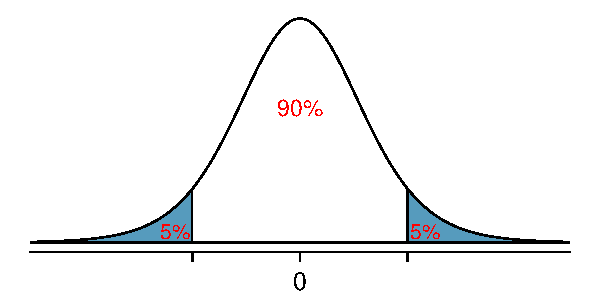
\includegraphics[width=\textwidth]{7-3_diff_two_mean/figures/middle90/middle90}
}
}

\end{frame}

%%%%%%%%%%%%%%%%%%%%%%%%%%%%%%%%%%%%

\begin{frame}[fragile]
\frametitle{臨界値}

\pq{0.99カラットと1カラットのダイヤモンドの平均ポイント価格の差に対する信頼区間に適切な$t^\star$はどれか？}

\begin{enumerate}[(a)]
\item 1.32
\solnMult{1.72}
\item 2.07
\item 2.82
\end{enumerate}


\begin{verbatim}
> qt(p = 0.95, df = 22)

[1] 1.717144
\end{verbatim}


\end{frame}

%%%%%%%%%%%%%%%%%%%%%%%%%%%%%%%%%%%%

\begin{frame}
\frametitle{信頼区間}

\dq{区間を計算し、文脈の中で解釈せよ。}

\soln{
\[ \text{点推定量} \pm ME \]
\begin{eqnarray*}
(\bar{x}_{pt99} - \bar{x}_{pt1}) \pm t^\star_{df} \times SE &=& (44.50 - 53.43) \pm 1.72 \times 3.56 \\
&=& -8.93 \pm  6.12 \\
&=& (-15.05, -2.81)
\end{eqnarray*}
0.99カラットのダイヤモンドの平均ポイント価格は1カラットの平均ポイント価格より\$15.05から\$2.81低いと90\%の信頼度で言える。
}

\end{frame}

%%%%%%%%%%%%%%%%%%%%%%%%%%%%%%%%%%%%

\subsection{まとめ}

%%%%%%%%%%%%%%%%%%%%%%%%%%%%%%%%%%%%

\begin{frame}
\frametitle{まとめ：2つの小標本平均の差を用いた推測}

\begin{itemize}

\item $\sigma_1$または$\sigma_2$が未知の場合、標本平均の差は$SE = \sqrt{ \frac{s_1^2}{n_1} + \frac{s_2^2}{n_1} }$の$t$分布に従う。

\item 条件：
\begin{itemize}
\item グループ内の独立性（ランダムサンプルで確認、非復元抽出の場合は$n < $母集団の10\%）とグループ間の独立性
\item いずれのグループにも極端な歪みがない
\end{itemize}

\item 仮説検定：
\[ T_{df} = \frac{\text{点推定量} - \text{帰無値}}{SE}\text{，ただし }df = \min(n_1 - 1, n_2 - 1) \]

\item 信頼区間：
\[ \text{点推定量} \pm t_{df}^\star \times SE \]

\end{itemize}

\end{frame}

%%%%%%%%%%%%%%%%%%%%%%%%%%%%%%%%%%%

%%%%%%%%%%%%%%%%%%%%%%%%%%%%%%%%%%%%

\section{2標本検定の検出力の計算}

%%%%%%%%%%%%%%%%%%%%%%%%%%%%%%%%%%%%

\begin{frame}
\frametitle{}

\begin{center}
\begin{tabular}{l l | c c}
\multicolumn{2}{c}{} & \multicolumn{2}{c}{\textbf{決定}} \\
& & $H_0$を棄却しない &  $H_0$を棄却する \\
  \cline{2-4}
& $H_0$が真 & \green{$1 - \alpha$} & \orange{第一種の過誤，$\alpha$} \\
\raisebox{1.5ex}{\textbf{真実}} & $H_A$が真 &  \orange{第二種の過誤，$\beta$} & \green{検出力，$1 - \beta$} \\
  \cline{2-4}
\end{tabular}
\end{center}

\begin{itemize}
\item 第一種の過誤は$H_0$を誤って棄却することであり、その確率は$\alpha$（有意水準）である。

\item 第二種の過誤は$H_0$を棄却すべきときに棄却しないことであり、その確率は$\beta$（計算は少し複雑）である。

\item 検定の\hl{検出力}は$H_0$を正しく棄却する確率であり、その確率は$1 - \beta$である。

\item 仮説検定では$\alpha$と$\beta$を低く保ちたいが、両者の間にはトレードオフが存在する。

\end{itemize}

\end{frame}

%%%%%%%%%%%%%%%%%%%%%%%%%%%%%%%%%%%%

\begin{frame}
\frametitle{第二種の過誤の確率}

対立仮説が実際に真である場合、第二種の過誤（棄却すべきときに帰無仮説を棄却しない）を犯す可能性はどれくらいか？

\begin{itemize}

\item 答えは自明ではない。

\item 真の母集団平均が帰無仮説の値に非常に近い場合、差を検出する（$H_0$を棄却する）のが難しい。

\item 真の母集団平均が帰無仮説の値から大きく離れている場合、差を検出しやすい。

\item 明らかに、$\beta$は\hl{効果量}（$\delta$）に依存する。
\end{itemize}

\end{frame}

%%%%%%%%%%%%%%%%%%%%%%%%%%%%%%%%%%%%

\begin{frame}
\frametitle{例 - 血圧（BP）：仮説}

{\dq
{\footnotesize
ある製薬会社が血圧を下げる新薬を開発し、臨床試験でその有効性を検証しようとしているとする。特定の標準的な血圧薬を服用している人々を募集し、被験者の半分に新薬（治療群）を投与し、残りの半分には外見が同じプラセボで現在の薬を継続服用させる（対照群）。この文脈での両側仮説検定の仮説は何か？
}
}

\soln{
\begin{align*}
H_0&: \mu_{\text{治療群}} - \mu_{\text{対照群}} = 0 \\
H_A&: \mu_{\text{治療群}} - \mu_{\text{対照群}} \ne 0
\end{align*}
}

\end{frame}

%%%%%%%%%%%%%%%%%%%%%%%%%%%%%%%%%%%%

\begin{frame}
\frametitle{例 - BP：標準誤差}

{\dq
{\footnotesize
研究者は収縮期血圧が140から180 mmHgの患者を対象に臨床試験を行うとする。以前発表された研究によれば、患者の血圧の標準偏差は約12 mmHgで、分布はほぼ対称であるとする。グループごとに100人の患者がいる場合、治療群と対照群の標本平均の差の近似標準誤差はどれくらいか？
}
}

\soln{
\[ SE = \sqrt{ \frac{12^2}{100} + \frac{12^2}{100} } = 1.70 \]
}

\end{frame}

%%%%%%%%%%%%%%%%%%%%%%%%%%%%%%%%%%%%

\begin{frame}
\frametitle{例 - BP：$H_0$を棄却するために必要な最小効果量}

{\dq
{\footnotesize
5\%の有意水準で帰無仮説を棄却するためには、治療群と対照群の観察された血圧平均の差（効果量）はどの値である必要があるか？}
}

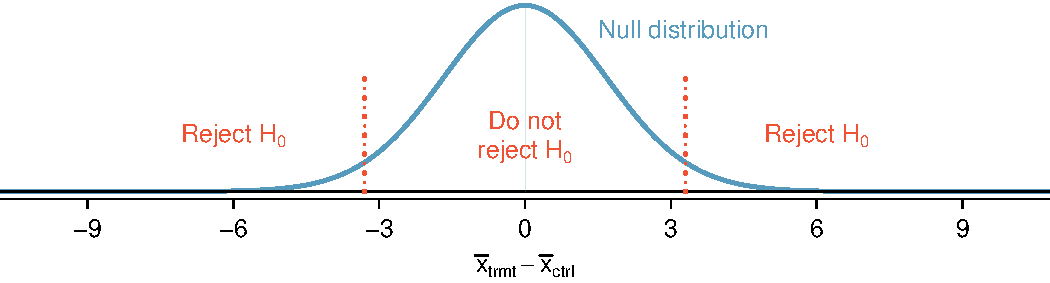
\includegraphics[width=\textwidth]{7-4_power/figures/power/power_null_B_0_1-7_with_rejection_region}

差は少なくとも
\[ 1.96 \times 1.70 = 3.332 \]
または多くとも
\[ -1.96 \times 1.70 = -3.332 \]
である必要がある。

\end{frame}

%%%%%%%%%%%%%%%%%%%%%%%%%%%%%%%%%%%%

\begin{frame}
\frametitle{例 - BP：検出力}

{\dq
{\footnotesize
研究者が標準薬と比べて3 mmHg以上の血圧への影響を検出することに関心があるとする。この効果を検出できる検定の検出力はどれくらいか？
}}

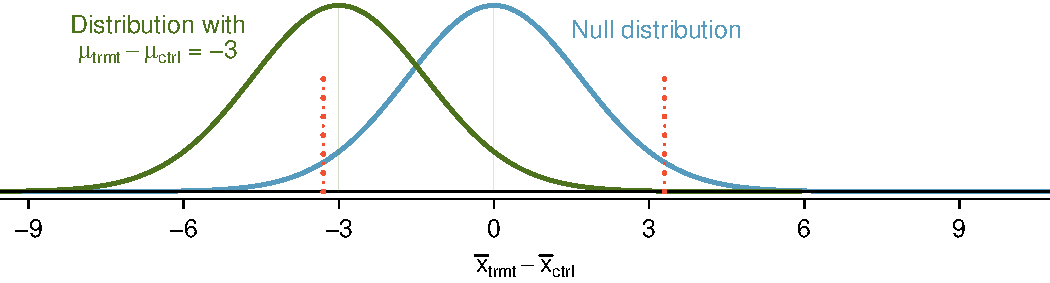
\includegraphics[width=\textwidth]{7-4_power/figures/power/power_null_C_0_1-7_with_alt_at_3}

\[ Z = \frac{-3.332 - (-3)}{1.70} = -0.20 \]

\[ P(Z < -0.20) = 0.4207 \]

\end{frame}

%%%%%%%%%%%%%%%%%%%%%%%%%%%%%%%%%%%%

\begin{frame}
\frametitle{例 - BP：80\%の検出力に必要な標本サイズ}

{\dq
{\footnotesize
この検定で80\%の検出力を得るためにはどれくらいの標本サイズが必要か？
}}

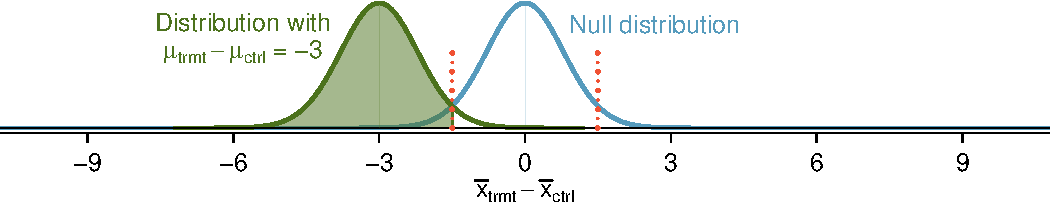
\includegraphics[width=\textwidth]{7-4_power/figures/power/power_null_0_0-76_with_alt_at_3_and_shaded}

\[ SE = \frac{3}{2.8} = 1.07142 \]

\[ 1.07142 = \sqrt{ \frac{12^2}{n} + \frac{12^2}{n} } \]

\[ n = 250.88 \rightarrow n \ge 251 \]

\end{frame}

%%%%%%%%%%%%%%%%%%%%%%%%%%%%%%%%%%%%

\begin{frame}
\frametitle{まとめ}

\begin{itemize}
\item 目標の検出力のレベルに必要な標本サイズを計算する。
\item 様々な標本サイズに対して検出力を計算し、目標の検出力（通常80\%または90\%）が得られる標本サイズを選ぶ。
\end{itemize}
\begin{center}
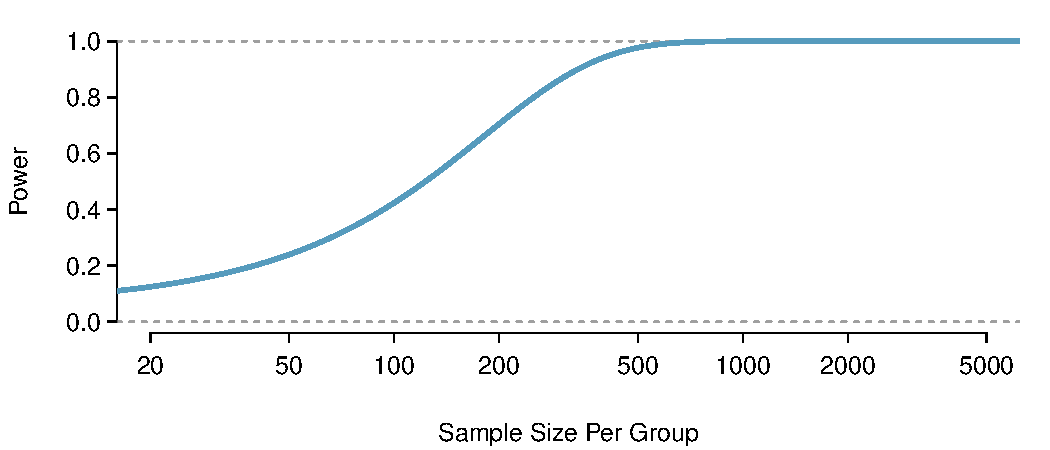
\includegraphics[width=0.7\textwidth]{7-4_power/figures/power/power_curve_neg-3}
\end{center}

\end{frame}

%%%%%%%%%%%%%%%%%%%%%%%%%%%%%%%%%%%%

\begin{frame}
\frametitle{望ましい検出力を達成する方法}

検出力を高める（第二種の過誤率を下げる）方法はいくつかある：

{\small
\begin{enumerate}

\item 標本サイズを増やす。

\item 標本の標準偏差を減らす。これは実質的に標本サイズを増やすのと同じ効果をもたらす（標準誤差が小さくなる）。$s$が小さいほど、帰無値と観察された点推定量を区別しやすくなる。確保するのは難しいが、慎重な測定プロセスと母集団をより均質に限定することで助けになる場合がある。

\item $\alpha$を増やすことで$H_0$を棄却しやすくする（ただし、これには第一種の過誤率が増加するという副作用がある）。

\item より大きな効果量を考慮する。母集団の真の平均が対立仮説にあるが帰無値に近い場合、差を検出するのが難しくなる。

\end{enumerate}
}

\end{frame}

%%%%%%%%%%%%%%%%%%%%%%%%%%%%%%%%%%%%

%%%%%%%%%%%%%%%%%%%%%%%%%%%%%%%%%%

\section{ANOVAによる平均の比較}

%%%%%%%%%%%%%%%%%%%%%%%%%%%%%%%%%%%

\subsection{ウルフ川のアルドリン}

%%%%%%%%%%%%%%%%%%%%%%%%%%%%%%%%%%%

\begin{frame}
\frametitle{}

\begin{center}
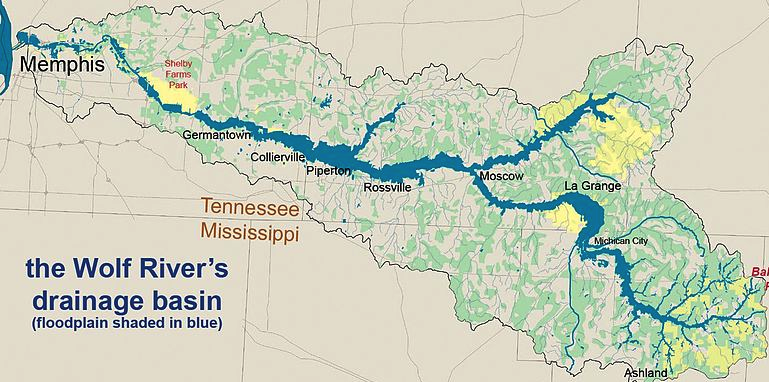
\includegraphics[width=0.5\textwidth]{7-5_anova/figures/aldrin/wolf}
\end{center}

{\small
\begin{itemize}

\item テネシー州のウルフ川は、殺虫剤産業がクロルダン（農薬）、アルドリン、ディエルドリン（いずれも殺虫剤）などの廃棄物を捨てていたかつての廃棄場跡地のそばを流れている。

\item これらの高毒性有機化合物は、様々な種類のがんや先天性異常を引き起こす可能性がある。

\item これらの物質が川に存在するかどうかを検定する標準的な方法は、深さの10分の6の深さで採取することである。

\item しかし、これらの化合物は水よりも密度が高く、分子が堆積粒子に付着する傾向があるため、中深度よりも底部付近でより高い濃度で見られる可能性が高い。

\end{itemize}
}

\end{frame}

%%%%%%%%%%%%%%%%%%%%%%%%%%%%%%%%%%%

\begin{frame}
\frametitle{データ}

3つの深さレベルでのアルドリン濃度（ナノグラム/リットル）。\\

\begin{center}
\begin{tabular}{r | c | c}
\hline
 	& アルドリン 					& 深さ \\
\hline
1 	& \textcolor{darkGray}{3.80} 	& \textcolor{darkGray}{底部}  \\
2 	& \textcolor{darkGray}{4.80} 	& \textcolor{darkGray}{底部}  \\
...	&						& \\
10	& \textcolor{darkGray}{8.80} 	& \textcolor{darkGray}{底部} \\
11	& \textcolor{blue}{3.20} 		& \textcolor{blue}{中深度}  \\
12	& \textcolor{blue}{3.80} 		& \textcolor{blue}{中深度} \\
...	&						& \\
20 	& \textcolor{blue}{6.60} 		& \textcolor{blue}{中深度} \\
21	& \textcolor{oiB}{3.10} 		& \textcolor{oiB}{表面} \\
22	& \textcolor{oiB}{3.60} 		& \textcolor{oiB}{表面} \\
...	&						& \\
30 	& \textcolor{oiB}{5.20} 		& \textcolor{oiB}{表面} \\
\hline
\end{tabular}
\end{center}

\end{frame}

%%%%%%%%%%%%%%%%%%%%%%%%%%%%%%%%%%%

\begin{frame}
\frametitle{探索的分析}

3つの深さレベルでのアルドリン濃度（ナノグラム/リットル）。\\

\begin{center}
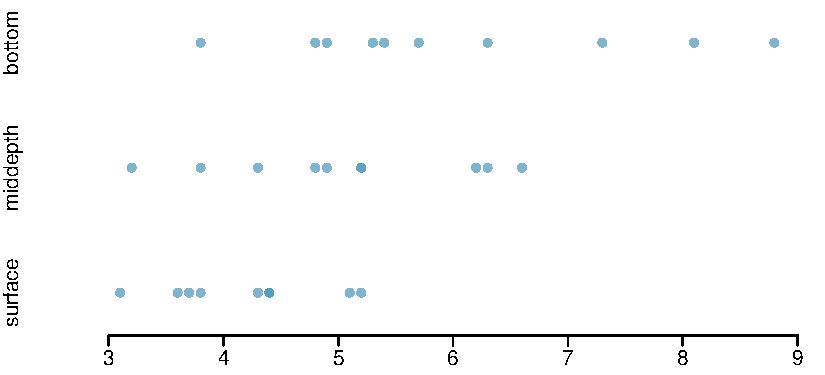
\includegraphics[width=0.75\textwidth]{7-5_anova/figures/aldrin/dotplot}
\end{center}

\begin{center}
\begin{tabular}{l | c c c}
		& n	& 平均	& 標準偏差	\\
\hline
底部	& 10	& 6.04	& 1.58 \\
中深度	& 10	& 5.05	& 1.10 \\
表面	& 10	& 4.20	& 0.66 \\
\hline
全体	& 30	& 5.10	& 1.37
\end{tabular}
\end{center}

\end{frame}

%%%%%%%%%%%%%%%%%%%%%%%%%%%%%%%%%%%

\begin{frame}
\frametitle{研究の問い}

\dq{3つの深さレベル間でアルドリン濃度の平均に差があるか？}

\vspace{0.5cm}

\begin{itemize}

\item 2グループの平均を比較するには$Z$または$T$統計量を使う。

\item 3グループ以上の平均を比較するには、\hl{ANOVA（分散分析）}という新しい検定と\hl{$F$}という新しい統計量を使う。

\end{itemize}

\end{frame}

%%%%%%%%%%%%%%%%%%%%%%%%%%%%%%%%%%%

\begin{frame}
\frametitle{ANOVA（分散分析）}

ANOVAは、目的変数の平均がカテゴリ変数の異なるレベルで異なるかどうかを評価するために使われる。

\begin{itemize}
\item[] \mathhl{H_0:} すべてのカテゴリで目的変数の平均は同じである。
\[\mu_1 = \mu_2 = \cdots = \mu_k, \]
ここで$\mu_i$はカテゴリ$i$の観測値の目的変数の平均を表す。
\item[]
\item[] \mathhl{H_A:} 少なくとも1つの平均が他と異なる。
\end{itemize}

\end{frame}

%%%%%%%%%%%%%%%%%%%%%%%%%%%%%%%%%%%

\begin{frame}
\frametitle{条件の確認}

\begin{enumerate}

\item 観測値はグループ内およびグループ間で独立でなければならない。

\begin{itemize}
\item データが母集団の10\%未満の単純無作為標本であれば、この条件は満たされる。
\item データが独立かどうかを注意深く考える（例えば、対になっていないか）。
\item 常に重要だが、確認が難しい場合もある。
\end{itemize}

\item 各グループ内の観測値はほぼ正規分布に従う必要がある。

\begin{itemize}
\item 標本サイズが小さい場合に特に重要である。
\end{itemize}

\dq{正規性はどのように確認するか？}

\item グループ間の変動性はほぼ等しい必要がある。

\begin{itemize}
\item グループ間で標本サイズが異なる場合に特に重要である。
\end{itemize}

\dq{この条件はどのように確認できるか？}

\end{enumerate}

\end{frame}

%%%%%%%%%%%%%%%%%%%%%%%%%%%%%%%%%%%

\begin{frame}
\frametitle{$z$/$t$検定 vs. ANOVA - 目的}

\twocol{0.5}{0.5}
{
\[ \hl{$z$/$t$検定} \]
\hl{2つ}のグループの平均を比較し、観察された差がサンプリング変動によって合理的に説明できないほど離れているかどうかを見る。
\[ H_0: \mu_1 = \mu_2 \]
}
{
\[ \hl{ANOVA} \]
\hl{2つ以上}のグループの平均を比較し、観察された差がすべてサンプリング変動によって合理的に説明できないほど離れているかどうかを見る。
\[ H_0: \mu_1 = \mu_2 = \cdots = \mu_k \]
}

\end{frame}

%%%%%%%%%%%%%%%%%%%%%%%%%%%%%%%%%%%

\begin{frame}
\frametitle{$z$/$t$検定 vs. ANOVA - 方法}

\twocol{0.5}{0.5}
{
\[ \hl{$z$/$t$検定} \]
検定統計量（比）を計算する。
\[ z / t = \frac{(\bar{x}_1 - \bar{x}_2) - (\mu_1 - \mu_2)}{SE(\bar{x}_1 - \bar{x}_2)} \]
}
{
\[ \hl{ANOVA} \]
検定統計量（比）を計算する。
\[ F = \frac{\text{群間変動}}{\text{群内変動}} \]
}

\vspace{1cm}

\begin{itemize}

\item 大きな検定統計量は小さなp値をもたらす。

\item p値が十分小さければ$H_0$は棄却され、母集団平均は等しくないと結論付ける。

\end{itemize}

\end{frame}

%%%%%%%%%%%%%%%%%%%%%%%%%%%%%%%%%%%

\begin{frame}
\frametitle{$z$/$t$検定 vs. ANOVA}

\begin{itemize}

\item グループが2つだけの場合、検定統計量の分母にプールされた分散を使えば$t$検定とANOVAは等価となる。

\item グループが3つ以上の場合、ANOVAは標本平均を全体の\hl{総平均}と比較する。

\end{itemize}

\end{frame}

%%%%%%%%%%%%%%%%%%%%%%%%%%%%%%%%%%%

\begin{frame}
\frametitle{仮説}

\pq{3つの深さレベル間でアルドリン濃度の平均に差があるかを検定するための正しい仮説はどれか？}

\begin{enumerate}[(a)]
\item $H_0: \mu_B = \mu_M = \mu_S$ \\
$H_A: \mu_B \ne \mu_M \ne \mu_S$ \\
\item $H_0: \mu_B \ne \mu_ M \ne \mu_S$ \\
$H_A: \mu_B = \mu_M = \mu_S$ \\
\solnMult{$H_0: \mu_B = \mu_M = \mu_S$ \\
$H_A:$ 少なくとも1つの平均が他と異なる。}
\item $H_0: \mu_B = \mu_M = \mu_S = 0$ \\
$H_A:$ 少なくとも1つの平均が他と異なる。
\item $H_0: \mu_B = \mu_M = \mu_S$ \\
$H_A: \mu_B > \mu_M > \mu_S$ \\
\end{enumerate}

\end{frame}

%%%%%%%%%%%%%%%%%%%%%%%%%%%%%%%%%%%

\subsection{ANOVAとF検定}

%%%%%%%%%%%%%%%%%%%%%%%%%%%%%%%%%%%

\begin{frame}
\frametitle{検定統計量}

\dq{グループ内の変動は大きく見えるか？グループ間はどうか？}

\[ F = \frac{\text{群間変動}}{\text{群内変動}}  \]

\begin{center}
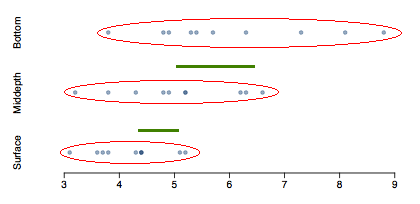
\includegraphics[width=0.75\textwidth]{7-5_anova/figures/aldrin/dotplot_var}
\end{center}

\end{frame}

%%%%%%%%%%%%%%%%%%%%%%%%%%%%%%%%%%%

\begin{frame}
\frametitle{$F$分布とp値}

\[ F =  \frac{\text{群間変動}}{\text{群内変動}} \]

\vspace{-1cm}

\begin{center}
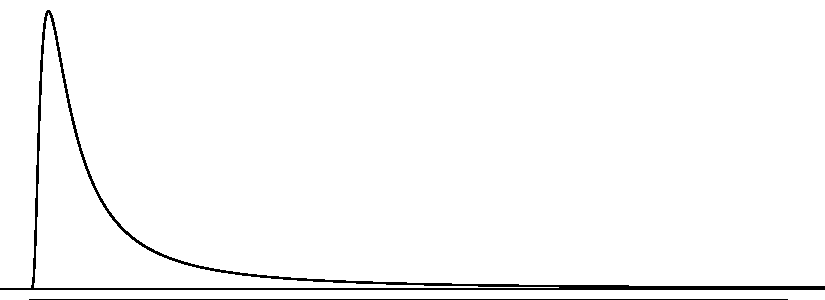
\includegraphics[width=0.75\textwidth]{7-5_anova/figures/fdist/fdist}
\end{center}

\begin{itemize}

\item $H_0$を棄却するためには小さなp値が必要であり、そのためには大きな$F$統計量が必要である。

\item 大きな$F$統計量を得るためには、標本平均間の変動がグループ内の変動よりも大きい必要がある。

\end{itemize}

\end{frame}

%%%%%%%%%%%%%%%%%%%%%%%%%%%%%%%%%%%

\subsection{ANOVA出力の解説}

%%%%%%%%%%%%%%%%%%%%%%%%%%%%%%%%%%%

\begin{frame}
\frametitle{}

\vspace{-0.5cm}

{\footnotesize
\begin{center}
\begin{tabular}{ll >{\columncolor[gray]{.6}[.5\tabcolsep]}rrrrr}
\hline
 			& 			& Df 	& Sum Sq	& Mean Sq 	& F value 	& Pr($>$F) \\
\hline
(\hl{G}roup) 	& depth 		& 2 	& 16.96 	& 8.48 		& 6.13 	& 0.0063 \\
(\hl{E}rror) 	& Residuals 	& 27 	& 37.33 	& 1.38 		&  		&  \\
\hline
	 		& \hl{T}otal	& 29	& 54.29 \\
\end{tabular}
\end{center}
}

\formula{ANOVAに関連する自由度}
{
\begin{itemize}
\item グループ：$df_G = k - 1$，ここで$k$はグループ数
\item 全体：$df_T = n - 1$，ここで$n$は総標本サイズ
\item 誤差：$df_E = df_T - df_G$
\end{itemize}
}

\begin{itemize}

\item $df_G = k - 1 = 3 - 1 = 2$ \\

\item $df_T = n - 1 = 30 - 1 = 29$

\item $df_E = 29 - 2 = 27$ \\

\end{itemize}

\end{frame}

%%%%%%%%%%%%%%%%%%%%%%%%%%%%%%%%%%%

\begin{frame}
\frametitle{}

\vspace{-0.25cm}

{\footnotesize
\begin{center}
\begin{tabular}{ll r>{\columncolor[gray]{.6}[.5\tabcolsep]}rrrr}
\hline
 			& 			& Df 	& Sum Sq	& Mean Sq 	& F value 	& Pr($>$F) \\
\hline
(\hl{G}roup) 	& depth 		& 2 	& \orange{16.96} 	& 8.48 		& 6.13 	& 0.0063 \\
(\hl{E}rror) 	& Residuals 	& 27 	& 37.33 	& 1.38 		&  		&  \\
\hline
	 		& \hl{T}otal	& 29	& 54.29 \\
\end{tabular}
\end{center}
}

\formula{グループ間の平方和，SSG}
{
グループ間の変動を測る
\vspace{-0.25cm}
\[ SSG = \sum_{i = 1}^{k} n_i (\bar{x}_i - \bar{x})^2 \]
ここで$n_i$は各グループサイズ，$\bar{x}_i$は各グループの平均，$\bar{x}$は全体（総）平均。
}

\vspace{-0.5cm}

\twocol{0.4}{0.5}
{
{\small
\begin{center}
\begin{tabular}{l | c c }
		& n	& 平均		\\
\hline
底部	& 10	& 6.04	 \\
中深度	& 10	& 5.05	 \\
表面	& 10	& 4.2	 \\
\hline
全体	& 30	& 5.1
\end{tabular}
\end{center}
}
}
{
\begin{eqnarray*}
SSG &=& \pr{ 10 \times (6.04 - 5.1)^2 } \\
&+& \pr{ 10 \times (5.05 - 5.1)^2 } \\
&+& \pr{ 10 \times (4.2 - 5.1)^2 } \\
&=& 16.96 \\
\end{eqnarray*}
}

\end{frame}

%%%%%%%%%%%%%%%%%%%%%%%%%%%%%%%%%%%

\begin{frame}
\frametitle{}

\vspace{-0.25cm}

{\footnotesize
\begin{center}
\begin{tabular}{ll r>{\columncolor[gray]{.6}[.5\tabcolsep]}rrrr}
\hline
 			& 			& Df 	& Sum Sq	& Mean Sq 	& F value 	& Pr($>$F) \\
\hline
(\hl{G}roup) 	& depth 		& 2 	& 16.96	& 8.48 		& 6.13 	& 0.0063 \\
(\hl{E}rror) 	& Residuals 	& 27 	& 37.33 	& 1.38 		&  		&  \\
\hline
	 		& \hl{T}otal	& 29	& \orange{54.29} \\
\end{tabular}
\end{center}
}

\formula{全体の平方和，SST}
{
全体の変動を測る
\vspace{-0.25cm}
\[ SST = \sum_{i = 1}^{n} (x_i - \bar{x})^2 \]
ここで$x_i$はデータセットの各観測値を表す。
}

\vspace{-0.75cm}

{\small
\begin{eqnarray*}
SST &=& (3.8 - 5.1)^2 + (4.8 - 5.1)^2 + (4.9 - 5.1)^2 + \cdots + (5.2 - 5.1)^2 \\
&=& (-1.3)^2 + (-0.3)^2 + (-0.2)^2 + \cdots + (0.1)^2 \\
&=& 1.69 + 0.09 + 0.04 + \cdots + 0.01 \\
&=& 54.29
\end{eqnarray*}
}

\end{frame}

%%%%%%%%%%%%%%%%%%%%%%%%%%%%%%%%%%%

\begin{frame}
\frametitle{}

\vspace{-0.25cm}

{\footnotesize
\begin{center}
\begin{tabular}{ll r>{\columncolor[gray]{.6}[.5\tabcolsep]}rrrr}
\hline
 			& 			& Df 	& Sum Sq	& Mean Sq 	& F value 	& Pr($>$F) \\
\hline
(\hl{G}roup) 	& depth 		& 2 	& 16.96	& 8.48 		& 6.13 	& 0.0063 \\
(\hl{E}rror) 	& Residuals 	& 27 	& \orange{37.33} 	& 1.38 		&  		&  \\
\hline
	 		& \hl{T}otal	& 29	& 54.29 \\
\end{tabular}
\end{center}
}

\formula{誤差の平方和，SSE}
{
グループ内の変動を測る：
\[ SSE = SST - SSG \]
}

\[ SSE =  54.29 - 16.96 =  37.33 \]

\end{frame}

%%%%%%%%%%%%%%%%%%%%%%%%%%%%%%%%%%%

\begin{frame}
\frametitle{}

\vspace{-0.25cm}

{\footnotesize
\begin{center}
\begin{tabular}{ll rr>{\columncolor[gray]{.6}[.5\tabcolsep]}rrr}
\hline
 			& 			& Df 	& Sum Sq	& Mean Sq 	& F value 	& Pr($>$F) \\
\hline
(\hl{G}roup) 	& depth 		& 2 	& 16.96	& \orange{8.48} 		& 6.13 	& 0.0063 \\
(\hl{E}rror) 	& Residuals 	& 27 	& 37.33 	& \orange{1.38} 		&  		&  \\
\hline
	 		& \hl{T}otal	& 29	& 54.29 \\
\end{tabular}
\end{center}
}

\formula{平均二乗誤差}
{
平均二乗誤差は平方和を自由度で割って計算される。
}

\begin{eqnarray*}
MSG &=& 16.96 / 2 = 8.48 \\
MSE &=& 37.33 / 27 = 1.38
\end{eqnarray*}

\end{frame}

%%%%%%%%%%%%%%%%%%%%%%%%%%%%%%%%%%%

\begin{frame}
\frametitle{}

\vspace{-0.25cm}

{\footnotesize
\begin{center}
\begin{tabular}{ll rrr>{\columncolor[gray]{.6}[.5\tabcolsep]}rr}
\hline
 			& 			& Df 	& Sum Sq	& Mean Sq 	& F value 	& Pr($>$F) \\
\hline
(\hl{G}roup) 	& depth 		& 2 	& 16.96	& 8.48 		& \orange{6.14} 	& 0.0063 \\
(\hl{E}rror) 	& Residuals 	& 27 	& 37.33 	& 1.38 		&  		&  \\
\hline
	 		& \hl{T}otal	& 29	& 54.29 \\
\end{tabular}
\end{center}
}

\formula{検定統計量，F値}
{
先に述べたように、F統計量はグループ間変動とグループ内変動の比である。
\[ F = \frac{MSG}{MSE} \]
}

\[ F = \frac{8.48}{1.38} = 6.14 \]

\end{frame}

%%%%%%%%%%%%%%%%%%%%%%%%%%%%%%%%%%%

\begin{frame}
\frametitle{}

\vspace{-0.25cm}

{\footnotesize
\begin{center}
\begin{tabular}{ll rrr>{\columncolor[gray]{.6}[.5\tabcolsep]}rr}
\hline
 			& 			& Df 	& Sum Sq	& Mean Sq 	& F value 	& Pr($>$F) \\
\hline
(\hl{G}roup) 	& depth 		& 2 	& 16.96	& 8.48 		& \orange{6.14} 	& 0.0063 \\
(\hl{E}rror) 	& Residuals 	& 27 	& 37.33 	& 1.38 		&  		&  \\
\hline
	 		& \hl{T}otal	& 29	& 54.29 \\
\end{tabular}
\end{center}
}

\formula{p値}
{
p値は、すべてのグループの平均が等しいとした場合に、「グループ間」変動と「グループ内」変動の比が観察された値以上となる確率である。自由度$df_G$と$df_E$のF曲線の下で観察されたF統計量より右側の面積として計算される。
}

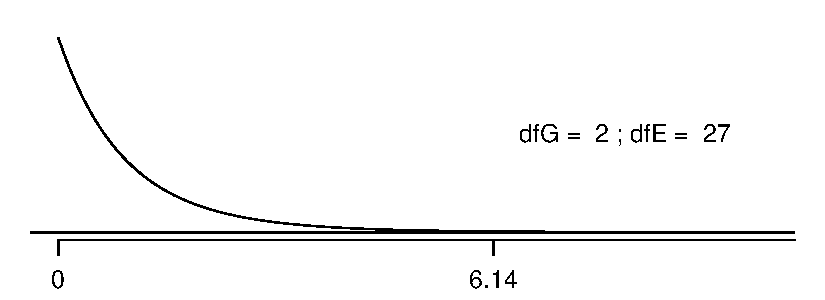
\includegraphics[width=0.9\textwidth]{7-5_anova/figures/aldrin/f}

\end{frame}

%%%%%%%%%%%%%%%%%%%%%%%%%%%%%%%%%%%

\begin{frame}
\frametitle{結論 - 文脈の中で}

\pq{仮説検定の結論は何か？}

$\:$ \\

データは、アルドリンの平均濃度が

\begin{enumerate}[(a)]

\item すべてのグループで異なることの説得力ある証拠を提供している。

\item 表面では他のレベルよりも低いことの説得力ある証拠を提供している。

\solnMult{少なくとも1つのグループで異なることの説得力ある証拠を提供している。}

\item すべてのグループで同じであることの説得力ある証拠を提供している。

\end{enumerate}

\end{frame}

%%%%%%%%%%%%%%%%%%%%%%%%%%%%%%%%%%%

\begin{frame}
\frametitle{結論}

\begin{itemize}

\item p値が小さい（$\alpha$未満）場合、$H_0$を棄却する。データは少なくとも1つの平均が他と異なることの説得力ある証拠を提供している（ただし、どのグループが異なるかは分からない）。

\item p値が大きい場合、$H_0$を棄却しない。データは少なくとも1対の平均が互いに異なることの説得力ある証拠を提供しておらず、標本平均の観察された差はサンプリング変動（偶然）によるものと考えられる。

\end{itemize}

\end{frame}

%%%%%%%%%%%%%%%%%%%%%%%%%%%%%%%%%%%

\subsection{条件の確認}

%%%%%%%%%%%%%%%%%%%%%%%%%%%%%%%%%%%

\begin{frame}[fragile]
\frametitle{（1）独立性}

\dq{この条件は満たされているように見えるか？}

\soln{この研究では、アルドリン濃度が互いに独立でないと考える理由はない。}

\end{frame}

%%%%%%%%%%%%%%%%%%%%%%%%%%%%%%%%%%%

\begin{frame}[fragile]
\frametitle{（2）ほぼ正規}

\dq{この条件は満たされているように見えるか？}

\begin{center}
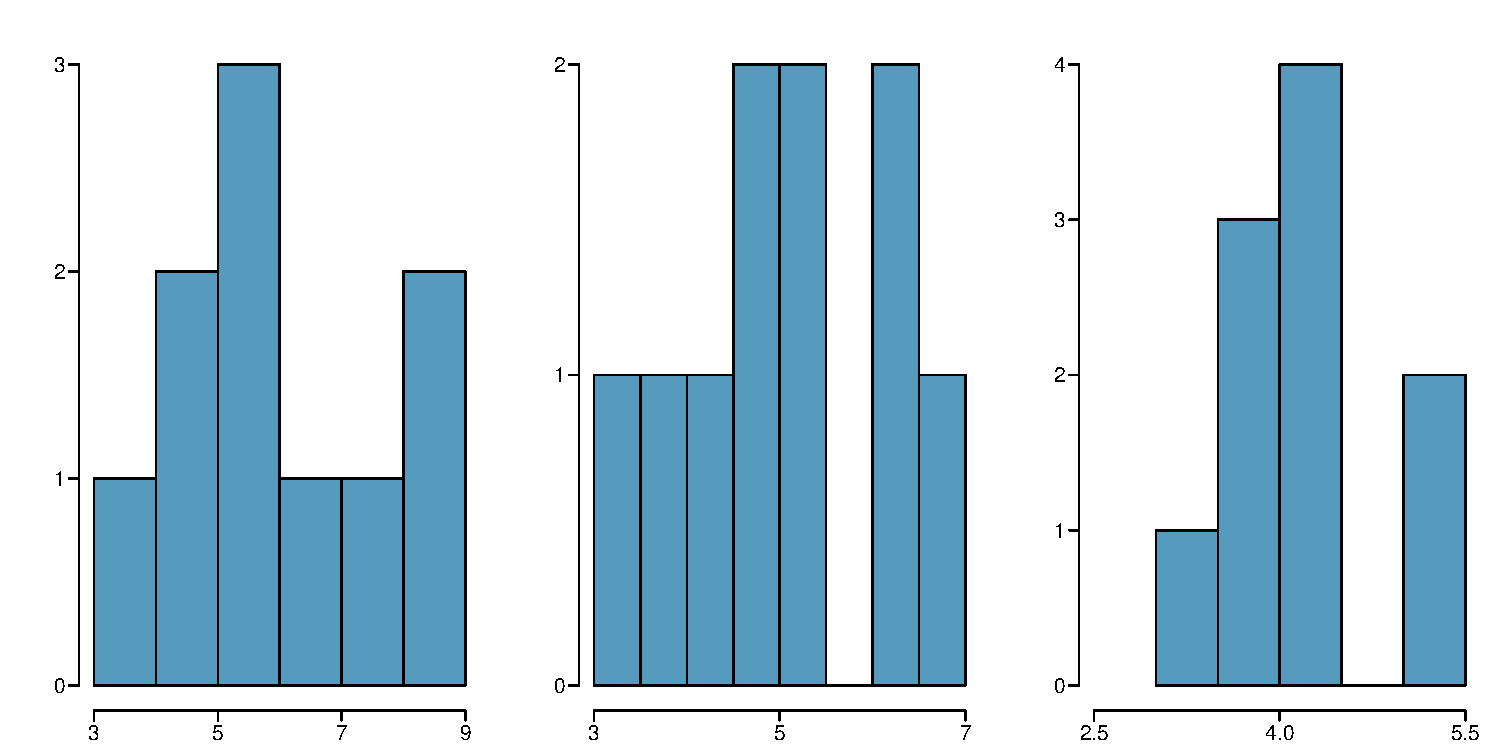
\includegraphics[width=\textwidth]{7-5_anova/figures/aldrin/normal}
\end{center}

\end{frame}

%%%%%%%%%%%%%%%%%%%%%%%%%%%%%%%%%%%

\begin{frame}[fragile]
\frametitle{（3）等分散性}

\dq{この条件は満たされているように見えるか？}

\begin{center}
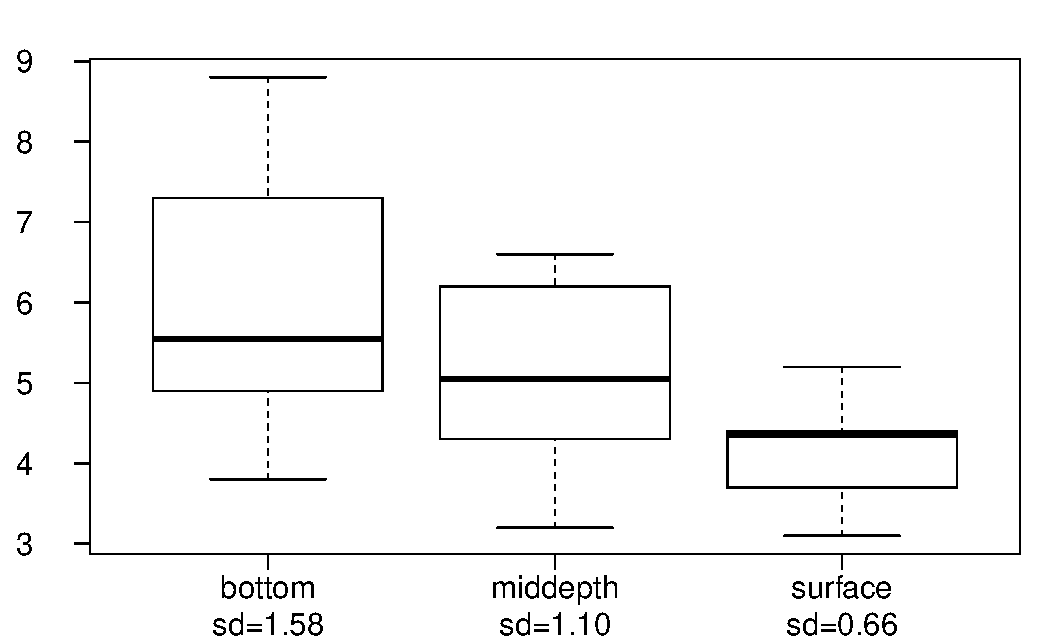
\includegraphics[width=0.7\textwidth]{7-5_anova/figures/aldrin/homo}
\end{center}

\end{frame}

%%%%%%%%%%%%%%%%%%%%%%%%%%%%%%%%%%%

\subsection{多重比較と第一種の過誤率}

%%%%%%%%%%%%%%%%%%%%%%%%%%%%%%%%%%%

\begin{frame}
\frametitle{どの平均が異なるか？}

\begin{itemize}

\item 先ほど少なくとも1対の平均が異なると結論付けた。自然に続く問いは「どの平均が？」である。

\item グループの全ての可能なペアについて2標本$t$検定を行うことができる。

\end{itemize}

\dq{このアプローチに潜在的な問題点は見えるか？}

\begin{itemize}

\item 多くの検定を行うと、第一種の過誤率が増加する。

\item この問題は修正された有意水準を使用することで解決される。

\end{itemize}

\end{frame}

%%%%%%%%%%%%%%%%%%%%%%%%%%%%%%%%%%%

\begin{frame}
\frametitle{多重比較}

\begin{itemize}

\item 多くのペアのグループを検定するこのシナリオを\hl{多重比較}（対比較）と呼ぶ。

\item \hl{ボンフェローニ補正}は、これらの検定にはより\orange{厳格な}有意水準が適切であることを示唆する：

\[ \alpha^\star = \alpha / K \]

ここで$K$は検討している比較の数である。

\item $k$グループがある場合、通常すべての可能なペアが比較され、$K = \frac{k (k - 1)}{2}$となる。

\end{itemize}

\end{frame}

%%%%%%%%%%%%%%%%%%%%%%%%%%%%%%%%%%%

\begin{frame}
\frametitle{修正$\alpha$の決定}

\pq{アルドリンデータセットでは深さに3つのレベル（底部、中深度、表面）がある。$\alpha = 0.05$の場合、どのペアの平均に有意差があるかを判断する2標本$t$検定の修正有意水準はどれであるべきか？}

\begin{enumerate}[(a)]
\item $\alpha^* = 0.05$
\item $\alpha^* = 0.05 / 2 = 0.025$
\solnMult{$\alpha^* = 0.05 / 3 = 0.0167$}
\item $\alpha^* = 0.05 / 6 = 0.0083$
\end{enumerate}

\end{frame}

%%%%%%%%%%%%%%%%%%%%%%%%%%%%%%%%%%%

\begin{frame}
\frametitle{どの平均が異なるか？}

\pq{以下の箱ひげ図に基づいて、どの平均が有意に異なると予想されるか？}

\twocol{0.6}{0.4}{
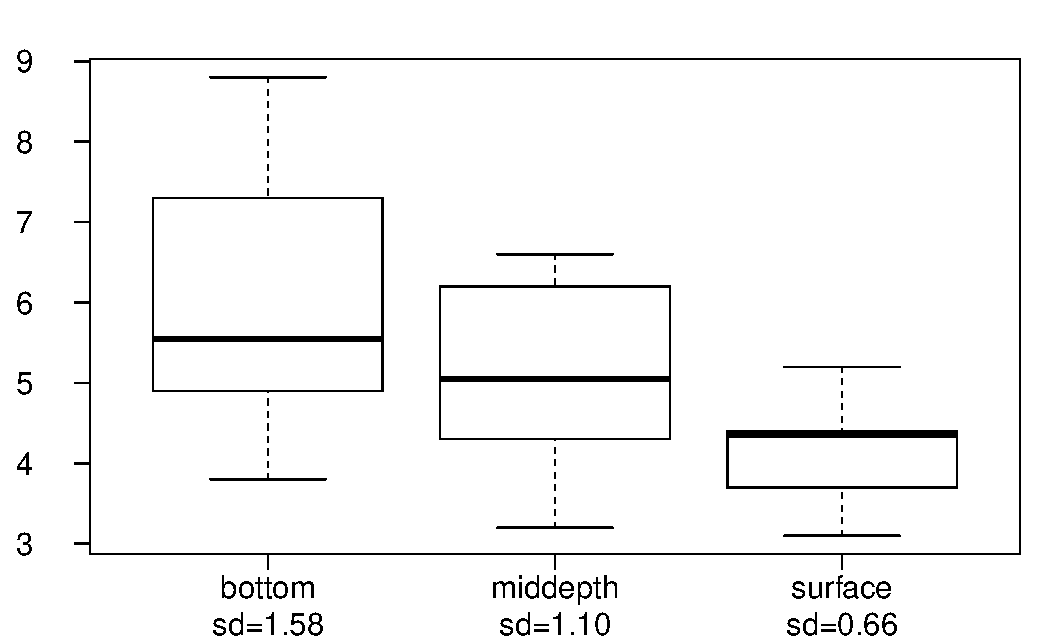
\includegraphics[width=\textwidth]{7-5_anova/figures/aldrin/homo}
}
{
\begin{enumerate}[(a)]
\item 底部 \& 表面
\item 底部 \& 中深度
\item 中深度 \& 表面
\item 底部 \& 中深度；中深度 \& 表面
\item 底部 \& 中深度；底部 \& 表面；中深度 \& 表面
\end{enumerate}
}

\end{frame}

%%%%%%%%%%%%%%%%%%%%%%%%%%%%%%%%%%

\begin{frame}
\frametitle{どの平均が異なるか？（続き）}

ANOVAのグループ間で等分散性の仮定が満たされる場合、すべてのグループのデータを使って変動性を推定できる：

\begin{itemize}

\item グループ内の標準偏差を$\sqrt{MSE}$（これが$s_{pooled}$）で推定する

\item $t$分布には誤差の自由度$n - k$を使う

\end{itemize}

\formula{2つの平均の差：ANOVA後}{
\[ SE = \sqrt{  \frac{\sigma_1^2}{n_1} + \frac{\sigma_2^2}{n_2} } \approx \sqrt{ \frac{MSE}{n_1} + \frac{MSE}{n_2} } \]
}

\end{frame}

%%%%%%%%%%%%%%%%%%%%%%%%%%%%%%%%%%

\begin{frame}[shrink=10]
\frametitle{}

\dq{底部と中深度での平均アルドリン濃度に差があるか？}

\twocol{0.4}{0.7}{
{\scriptsize
\begin{center}
\begin{tabular}{l | c c c}
		& n	& 平均	& 標準偏差	\\
\hline
底部	& 10	& \orange{6.04}	& 1.58 \\
中深度	& 10	& \orange{5.05}	& 1.10 \\
表面	& 10	& 4.2 	& 0.66 \\
\hline
全体	& 30	& 5.1		& 1.37
\end{tabular}
\end{center}
}
}
{
{\scriptsize
\begin{center}
\begin{tabular}{l rrrrr}
\hline
 			& Df 	& Sum Sq	& Mean Sq 	& F value 	& Pr($>$F) \\
\hline
depth 		& 2 	& 16.96 	& 8.48 		& 6.13 	& 0.0063 \\
Residuals 	& \orange{27} 	& 37.33 	& \orange{1.38} 		&  		&  \\
\hline
Total			& 29	& 54.29 \\
\end{tabular}
\end{center}
}
}

{\footnotesize
\begin{eqnarray*}
T_{df_E} &=& \frac{(\bar{x}_{\text{底部}} - \bar{x}_{\text{中深度}})}{\sqrt{ \tfrac{MSE}{n_{\text{底部}}} + \tfrac{MSE}{n_{\text{中深度}}} }} \\
T_{27} &=& \frac{( 6.04 - 5.05 )}{\sqrt{ \tfrac{1.38}{10} + \tfrac{1.38}{10} }} = \frac{0.99}{0.53}  =1.87 \\
0.05 &<& p\text{値} < 0.10 \quad \text{（両側）} \\
\alpha^\star &=& 0.05 / 3 = 0.0167
\end{eqnarray*}
}

{\small $H_0$を棄却しない。データは底部と中深度での平均アルドリン濃度に差がある説得力ある証拠を提供していない。}

\end{frame}

%%%%%%%%%%%%%%%%%%%%%%%%%%%%%%%%%%

\begin{frame}
\frametitle{}

\app{対比較}{底部と表面での平均アルドリン濃度に差があるか？}

\soln{
{\footnotesize
\begin{eqnarray*}
T_{df_E} &=& \frac{(\bar{x}_{\text{底部}} - \bar{x}_{\text{表面}})}{\sqrt{ \tfrac{MSE}{n_{\text{底部}}} + \tfrac{MSE}{n_{\text{表面}}} }} \\
T_{27} &=& \frac{( 6.04 - 4.2 )}{\sqrt{ \tfrac{1.38}{10} + \tfrac{1.38}{10} }} = \frac{1.84}{0.53}  =3.47 \\
p\text{値} = 0.0018 \qquad \text{（両側）} \\
\alpha^\star &=& 0.05 / 3 = 0.0167
\end{eqnarray*}
}
{\small $H_0$を棄却する。データは底部と表面での平均アルドリン濃度に差がある説得力ある証拠を提供している。}
}

\end{frame}

%%%%%%%%%%%%%%%%%%%%%%%%%%%%%%%%%%



%%%%%%%%%%%%%%%%%%%%%%%%%%%%%%%%%%%%
% ドキュメント終了
%%%%%%%%%%%%%%%%%%%%%%%%%%%%%%%%%%%%

\end{document}
